\chapter{Nützliche Shortcuts}\label{sec:shortcuts}

Mit Shortcuts können Sie Ihre Produktivität in vielen Bereichen boosten, daher empfiehlt es sich, diese zu lernen, ebenso wie das Zehn-Finger-System. Falls Sie letzteres noch nicht beherrschen, sollten Sie dieses zuerst auf einer Webseite wie beispielsweise \href{https://www.tipp10.com/de/}{tipp10.com} trainieren.

Folgende Shortcut-Auflistungen haben keinen Anspruch auf Vollständigkeit. Falls Sie weitere hilfreiche Shortcuts kennen, können Sie diese gerne an \href{mailto:\mainauthormailA}{\mainauthorA} oder \href{mailto:\mainauthorB}{\mainauthorB} senden. Sie dürfen die Übersicht der Shortcuts an jeder Prüfung verwenden.
\clearpage
\begin{multicols}{2}

	\begin{table}[H]
		\centering
		\footnotesize
		\begin{tabular}{p{3.7cm}||c|c}
			\textbf{Aktion}                                                                                                & \textbf{\faWindows{} Windows}                          & \textbf{\faApple{} MacOS}                   \\\midrule\midrule
			Cursor bew\textcolor{red!30}{\faICursor}\tikzmark{from1}e\tikzmark{to1}\textcolor{red}{\faICursor}gen          & \makecell{\keys{\arrowkeyright}, \keys{\arrowkeyleft}} & \keys{\arrowkeyright}, \keys{\arrowkeyleft} \\\midrule
			Cursor \textcolor{red!30}{\faICursor}\tikzmark{from2}bewegen\tikzmark{to2}\textcolor{red}{\faICursor} (Wörter) & \makecell{\keys{\ctrl+\arrowkeyright}                                                                \\\keys{\ctrl+\arrowkeyleft}} & \makecell{\keys{\Alt+\arrowkeyright}\\ \keys{\Alt+\arrowkeyleft}}\\\midrule
			\colorbox{RoyalBlue!50}{Wörter\faICursor} markieren                                                            & \makecell{\keys{\ctrl+\shift+\arrowkeyright}                                                         \\\keys{\ctrl+\shift+\arrowkeyleft}} & \makecell{\keys{\Alt+\shift+\arrowkeyright}\\ \keys{\Alt+\shift+\arrowkeyleft}}\\\midrule
			\makecell[l]{\faICursor Zum Anfang /                                                                                                                                                                                  \\Ende der Zeile gehen\faICursor} & \makecell{\keys{Home}\\\keys{End}}& \makecell{\keys{\cmd+\arrowkeyleft}\\\keys{\cmd+\arrowkeyright}}\\\midrule
			\colorbox{RoyalBlue!50}{Ganze Zeile markieren\faICursor}                                                       & \makecell{\keys{\shift+Home}                                                                         \\\keys{\shift+End}}& \makecell{\keys{\cmd+\shift+\arrowkeyleft}\\\keys{\cmd+\shift+\arrowkeyright}}\\\midrule
			\makecell[l]{\colorbox{RoyalBlue!50}{Gesamten Text}                                                                                                                                                                   \\\colorbox{RoyalBlue!50}{markieren}} &\keys{\ctrl + A}& \keys{\cmd + A}\\\midrule
			\emoji{smile} Emoji einfügen                                                                                   & \keys{\faWindows + .}                                  & \keys{fn + E}                               \\\midrule
			\faCopy{} Kopieren                                                                                             & \keys{\ctrl + C}                                       & \keys{\cmd + C}                             \\\midrule
			\makecell[l]{\faCut{} Ausschneiden                                                                                                                                                                                    \\(= kopieren + löschen)}&\keys{\ctrl + X}& \keys{\cmd + X}\\\midrule
			\faPaste{} Einfügen                                                                                            & \keys{\ctrl + V}                                       & \keys{\cmd + V}                             \\\midrule
			\faSearch{} Suchen                                                                                             & \keys{\ctrl + F}                                       & \keys{\cmd + F}                             \\\midrule
			\faSave{} Datei speichern                                                                                      & \keys{\ctrl + S}                                       & \keys{\cmd + S}                             \\\midrule
			\faUndo{} Rückgängig (``undo'')                                                                                & \keys{\ctrl + Z}                                       & \keys{\cmd + Z}                             \\\midrule
			\faRedo{} Vorwärts (``redo'')                                                                                  & \keys{\ctrl +\shift + Z}                               & \keys{\cmd + \shift + Z}                    \\\midrule
			\makecell[l]{\faArrowRight{} Fenster wechseln                                                                                                                                                                         \\\faArrowLeft{} Fenster zurückwechseln} & \makecell{\keys{\ctrl + \tabwin}\\\keys{\ctrl + \shift + \tabwin}} & \makecell{\keys{\cmd + \tab}\\\keys{\cmd + \shift + \tab}}\\\midrule
			\faWindowClose{} Programm schliessen                                                                           & \keys{\Alt + F4}                                       & \keys{\cmd + Q}                             \\\midrule
			\faLock{} Computer sperren                                                                                     & \keys{\faWindows + L}                                  & \keys{\cmd + \ctrl + Q}                     \\\midrule
			\makecell[l]{\faCaretLeft{} Fenster links anordnen                                                                                                                                                                    \\\faCaretRight{} Fenster rechts anordnen} &\makecell[l]{\keys{\faWindows+\arrowkeyleft}\\ \keys{\faWindows+\arrowkeyright}}& Nicht möglich \\
		\end{tabular}
		\caption{Allgemeine Shortcuts, funktionieren in fast jedem Programm}
	\end{table}

	\begin{tikzpicture}[overlay,remember picture]
		% Draw a 2D rectangle around the table title
		% draw arrow to title
		\draw[red,-stealth] (from1.south) to[bend right] (to1.south);
		\draw[red,-stealth] (from2.south) to[bend right] (to2.south);
	\end{tikzpicture}

	\begin{table}[H]
		\footnotesize
		\centering
		\begin{tabular}{c||c|c}
			\textbf{Aktion}                            & \textbf{\faWindows{} Windows} & \textbf{\faApple{} MacOS} \\\midrule\midrule
			\faCaretRight\faAlignLeft{} Code Einrücken & \keys{\tabwin}                & \keys{\tab}               \\\midrule
			\faAlignLeft\faCaretLeft{} Code Ausrücken  & \keys{\shift + \tabwin}       & \keys{\shift + \tab}      \\
		\end{tabular}
		\caption{Shortcuts für Code}
	\end{table}

	\begin{table}[H]
		\footnotesize
		\centering
		\begin{tabular}{p{2.3cm}||c|c}
			\textbf{Aktion}                                    & \textbf{\faWindows{} Windows} & \textbf{\faApple{} MacOS} \\\midrule\midrule
			\makecell[l]{\faArrowRight{} Tab nach rechts                                                                   \\\faArrowLeft{} Tab nach links} & \makecell{\keys{\ctrl + \tabwin}\\\keys{\ctrl + \shift + \tabwin}} & \makecell{\keys{\cmd+\Alt+\arrowkeyleft}\\\keys{\cmd+\Alt+\arrowkeyright}} \\\midrule
			\faArrowsAltH{} Zu Tab 1, 2, ... gehen             & \keys{\ctrl + zahl}           & \keys{\cmd + zahl}        \\\midrule
			\faWindowClose{} Tab schliessen                    & \keys{\ctrl + W}              & \keys{\cmd + W}           \\\midrule
			\faPlus{} Neuen Tab öffnen                         & \keys{\ctrl + T}              & \keys{\cmd + T}           \\\midrule
			\faWindowRestore{} Geschlossenen Tab wieder öffnen & \keys{\ctrl + \shift + T}     & \keys{\cmd + \shift + T}  \\\midrule
			\faRedo{} Seite neu laden                          & \keys{\ctrl + R}              & \keys{\cmd + R}           \\
		\end{tabular}
		\caption{Browser-Shortcuts}
	\end{table}

	\begin{table}[H]
		\footnotesize
		\centering
		\begin{tabular}{c||c|c}
			\textbf{Zeichen} & \textbf{\faWindows{} Windows} & \textbf{\faApple{} MacOS} \\\midrule\midrule
			$[$              & \keys{\AltGr+ü}               & \keys{\Alt+5}             \\\midrule
			$]$              & \keys{\AltGr+!}               & \keys{\Alt+6}             \\\midrule
			\{               & \keys{\AltGr+7}               & \keys{\Alt+8}             \\\midrule
			\}               & \keys{\AltGr+0}               & \keys{\Alt+9}             \\\midrule
			\textbackslash   & \keys{\AltGr+\textbackslash}  & \keys{\Alt+\shift+7}      \\\midrule
			\%               & \keys{\shift+5}               & \keys{\shift+5}           \\
		\end{tabular}
		\caption{Spezial-Zeichen}
	\end{table}
\end{multicols}\noindent\rule{\textwidth}{0.4pt}\begin{multicols}{2}
	\clearpage
	Viele weitere Shortcuts können erraten werden, indem man ausprobiert: Häufig steht der Anfangs-Buchstabe des englischen Wortes kurz für die Aktion. So kann man beispielsweise aus den meisten Programmen drucken (en. \textit{print}), indem man die Abkürzung \keys{\ctrl+P} auf Windows bzw. \keys{\cmd+P} auf MacOS verwendet. Bei MacOS können zudem viele Abkürzungen über das Menu des Programms (Menuleiste ganz oben am Bildschirm) eingesehen werden.
	\columnbreak
	\begin{figure}[H]
		\centering
		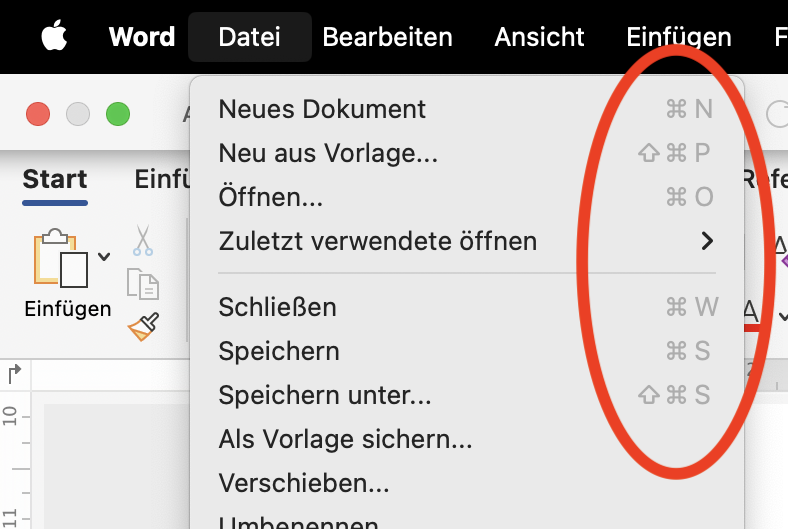
\includegraphics[width=0.7\linewidth]{GrundlagenInfo/00_Programmieren/Figures/shortcuts-macos}
	\end{figure}
\end{multicols}
